
\chapter{$\varepsilon$-次模逼近网络的影响力最大化}

在$\varepsilon$-次模逼近网络中,一些节点的阈值函数是$\varepsilon$-次模逼近而不再是次模函数,整体的影响力函数也不再有次模性质。
本章中会先讨论$\varepsilon$-次模逼近节点的个数是图节点个数多项式的时影响力最大化的不可近似性,
然后又设计了$\varepsilon$-次模逼近节点较少时的近似算法。

\section{$(\gamma,\varepsilon)$-ASIM的不可近似性}
本节我们会证明对于$n$个节点的图中,即使只有有$n$的多项式个$\varepsilon$-次模节点,
影响力最大化问题也很难近似。
下文用定理给出这个不可近似性的精确描述,然后本节接下来的部分会证明这个定理。


\subsection{不可近似性的主要结论}
\begin{theorem}
\label{the:inapp}
对于任意的$\varepsilon \in (0,1)$和任意的$\gamma \in (0,1)$,
在$(\gamma,\varepsilon)$-次模逼近图上不存在近似比为$1 / n^{\frac{\gamma}{c}}$的影响力最大化近似算法,
除非P=NP,这里$c = 3+3/\log{\frac{2}{2-\varepsilon}}$。
\end{theorem}

这个定理说明了只要图中有$n^{\gamma}$个$\varepsilon$-次模节点,不管$\gamma$有多少,影响力最大化问题都不能被近似。
不可近似的程度正比于$\gamma$的大小,$\gamma$越大,影响力最大化问题越难被近似。
定力的证明基于机关(gadget)的构造,我们通过二叉树级联机关构造出一个概率与门(probabilistic-AND gate),
然后我们通过NP完全问题Set Cover的规约证明了不可近似比的下界。

\subsection{基于二叉树的概率与门}
本小节介绍概率与门的构造和计算与门成功的概率。先介绍基础的机关,然后介绍通过二叉树级联得到的概率与门,最后计算与门的概率。


\begin{figure}[htbp]
\centering
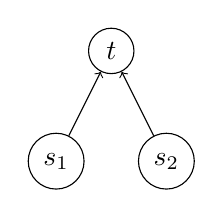
\begin{tikzpicture}[scale=0.7]
%\tikzstyle[thick]
\node at (1,2) [circle,draw](1) {$t$};
\node at (0,0) [circle,draw](2) {$s_1$};
\node at (2,0) [circle,draw](3) {$s_2$};
\path [->] (2) edge node{} (1);
\path [->] (3) edge node{} (1);
\end{tikzpicture}
\caption{基础机关结构}
\label{fig:gadget_basic}
\end{figure}
我们构建的机关如图\ref{fig:gadget_basic}所示,这个机关以节点$s_1,s_2$作为输入,以节点$t$作为输出。
节点$t$有两个入邻居,阈值函数$g(\cdot)$是$\varepsilon$-次模函数。
阈值函数$g(\cdot)$的赋值见等式\ref{eq:func_g}。
\begin{eqnarray*}
\label{eq:func_g}
g(S) =
\left\lbrace
\begin{aligned}
&0,		~ & |S|=0; \\
&\frac{1-\varepsilon}{2},	~ & |S|=1; \\
&1,		~ & |S|=2. \\
\end{aligned}
\right.
\end{eqnarray*}
函数$g(S)$的取值只依赖于输入集合的大小$|S|$,$g(\cdot)$被夹在两个线性的次模函数之间。
$g(\cdot)$自身是一个线性函数在$|S|=1$处向下偏移了$\varepsilon$。
这个基础机关距离与门的性质还很远,接下来我们介绍如何构造更复杂的机关。


我们希望构建出一个机关满足如下性质:
\begin{eqnarray*}
P_a(t) =
\left\lbrace
\begin{aligned}
&1,		~ & \mbox{$s_1,s_2$均被激活}; \\
&o(1),	~ & \mbox{$s_1,s_2$中只有一个被激活}; \\
&0,		~ & \mbox{$s_1,s_2$都未被激活}. \\
\end{aligned}
\right.
\end{eqnarray*}
其中$P_a(t)$是机关的输出节点$t$被激活的概率。
满足这样的性质,当输入节点$s_1,s_2$没有被全部激活时,输出节点$t$很大概率不会被激活。
前面的基础机关在$|S|=1$时,$t$被被激活的概率是$\frac{1-\varepsilon}{2}$,
我们做的就是通过二叉树级联机关放大$\frac{1-\varepsilon}{2}$和$\frac{1}{2}$的差距,
最终使得$|S|=1$时$t$很大概率不被激活,机关的构造如图\ref{fig:gadget_tree}所示。


\begin{figure}[htbp]
\centering
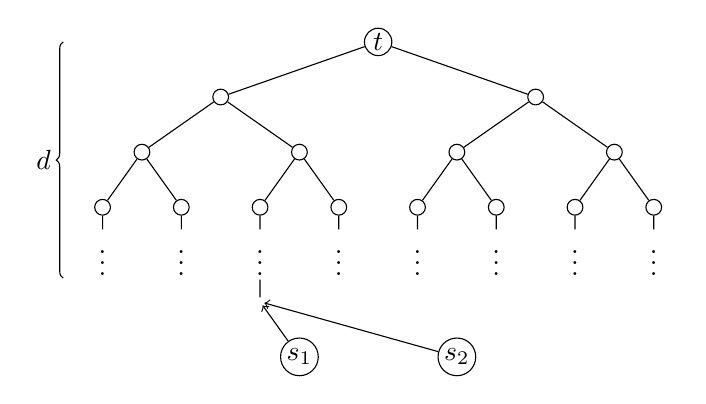
\begin{tikzpicture}[every node/.style={draw,circle,inner sep=1pt}]
% \draw[step=1cm, color=gray] (-5,-5) grid (5,5);
\tikzstyle{level 1}=[sibling distance=40mm,level distance=7mm]
\tikzstyle{level 2}=[sibling distance=20mm]
\tikzstyle{level 3}=[sibling distance=10mm]
\tikzstyle{level 4}=[level distance=6mm]
%\tikzstyle{level 5}=[sibling distance=15mm,level distance=10mm]
\draw[decorate, decoration={brace, mirror}] (-4cm, 0) -- (-4cm,-3cm);
\draw (-4.25cm, -1.5cm) node[draw=none] {$d$};

\node at (-1,-4) [circle,draw](2) {$s_1$};
\node at (1,-4) [circle,draw](3) {$s_2$};
\node {$t$}
	child{
		node{$~$}
		child{
			node{$~$}
			child{
				node{$~$}
				child{node[draw=none] {$\vdots$}
				}
			}
			child{
				node{$~$}
				child{node[draw=none]{$\vdots$}}
			}
		}
		child{
			node{$~$}
			child{
				node{$~$}
				child{node[draw=none]{$\vdots$}
					child{node[draw=none] (leaf_1) {$ $}}
				}
			}
			child{
				node{$~$}
				child{node[draw=none]{$\vdots$}
				}
			}
		}
	}
	child{
		node{$~$}
		child{
			node{$~$}
			child{
				node{$~$}
				child{node[draw=none]{$\vdots$}
				}
			}
			child{
				node{$~$}
				child{node[draw=none]{$\vdots$}}
			}
		}
		child{
			node{$~$}
			child{
				node{$~$}
				child{node[draw=none]{$\vdots$} }
			}
			child{
				node{$~$}
				child{node[draw=none] {$\vdots$}
					%child{node[draw=none] (leaf_2) {$ $}}
				}
			}
		}
	};

\path [->] (2) edge (leaf_1);
\path [->] (3) edge (leaf_1);
\end{tikzpicture}
\caption{二叉树机关$T_\varepsilon$}
\label{fig:gadget_tree}
\end{figure}

在这棵满二叉树中,输出节点$t$是二叉树的根节点,每个节点有一条有向边指向它的父节点。
对每个叶子结点$v$,输入节点$s_1,s_2$会发出有向边指向$v$。
二叉树中每个节点的阈值函数都是前文等式\ref{eq:func_g}定义的$\varepsilon$-次模函数$g(\cdot)$。
整个树状结构被定义为$T_\varepsilon$,$\varepsilon$就是函数$g(\cdot)$距离次模函数的偏移量。
二叉树的深度会在后文定义,我们用$v_i$表示深度为$i$的节点($t$的深度是$1$)。


很显然$s_1,s_2$都被激活时$P_a(t)=1$,$s_1$ or $s_2$都没有被激活时$P_a(t)=0$。
下面我们证明对于深度$d$的二叉树,$s_1,s_2$中只有一个被激活时,输出节点$t$被激活的概率是$O(2^{-d})$。
\begin{lemma}
\label{lem:tree_prob}
对于深度为$d$的机关$T_\varepsilon$,当输入节点只有一个被激活时,
输出节点$t$被激活的概率小于$(\frac{2-\varepsilon}{2})^{d}$。
\end{lemma}
\begin{proof}
对于所有的叶子结点$v_d$,可以得到$P_a(v_d) = \frac{1-\varepsilon}{2}$。
机关$T_\varepsilon$中同一层的节点之前激活与否是互相独立的。
给定一个基础机关(如图\ref{fig:gadget_basic}),如果每个输出节点被激活的概率都是$p$而且互相独立,则输出节点$t$被激活的概率是
\begin{equation*}
\begin{array}{ll}
& P_a(t) \\
= & p^2\times g(2) + 2p(1-p)\times g(1) + (1-p)^2\times g(0) \\
= & p^2 + 2p(1-p)\frac{1-\varepsilon}{2} = p(1-\varepsilon(1-p)).
\end{array}
\end{equation*}
根据这个公式,我们可以写出二叉树上不同深度节点被激活概率的递推公式。
\begin{equation}
\label{eq:recurrence}
P_a(v_i) = P_a(v_{i+1})(1-\varepsilon(1-P_a(v_{i+1}))) <  P_a(v_{i+1})(1-\varepsilon/2)
\end{equation}
不等号的成立是因为树的叶节点满足$P_a(v_d) = \frac{1-\varepsilon}{2}$,而且随着节点所处深度降低,被激活的概率递减。
所以对于树中的任意节点$v$都有$P_a(v) < \frac{1}{2}$。
根据递推公式\ref{eq:recurrence},输出节点$t$被激活的概率为
\begin{equation*}
\label{eq:p_a_t}
 P_a(t) 
=  P_a(v_1) 
<  \frac{1-\varepsilon}{2}(\frac{2-\varepsilon}{2})^{d-1} 
<  (\frac{2-\varepsilon}{2})^{d}.
\end{equation*}
节点$t$被激活的概率$P_a(t) = O(2^{-d})$,随着$d$的增加趋于$0$。
\end{proof}
由引理\ref{lem:tree_prob}我们知道$T_\varepsilon$在输入集合大小为$1$时输出节点被激活的概率是$o(1)$,
$T_\varepsilon$的确是一个两个输入节点的概率与门。
我们称概率与门在输入节点没有全部激活且输出节点保持未激活时为成功运作。


我们已经构造了两个输入节点的树状机关,我们拓展机关$T_\varepsilon$来得到$n$个输入节点的与门$T_\varepsilon^n$。
给定$n$个输入节点$s_1, s_2, \dots, s_n$,我们用节点$s_0$和$s_1$作为输入节点搭建$T_\varepsilon^n$,并令输出节点为$s_{12}$。
接下来可以把节点$s_{12}$和$s_{3}$作为输入节点搭建$T_\varepsilon^n$得到输出节点$s_{123}$。
以此类推,我们得到最终的输出节点$s_{12\dots n}$。
在这个结构中,$s_1, s_2, \dots, s_n$中有节点未被激活时,$s_{12\dots n}$很大概率不会被激活。
如果所有的$T_\varepsilon$都表现出与门的性质,那么整体上就构成了一个$n$个输入节点的概率与门。
由引理\ref{lem:tree_prob}可得深度为$d$的$T_\varepsilon$最多以$(\frac{2-\varepsilon}{2})^{d}$的概率不成功运作。
通过Union Bound,$T_\varepsilon^n$在输入中有未激活节点时输出节点被激活的概率至多为$n(\frac{2-\varepsilon}{2})^{d}$。
$T_\varepsilon^n$一共包含$n\times(2^d-1) = n2^d-n$个节点。



\subsection{基于Set Cover的不可近似性规约}
在本节基于概率与门,我们证明定理\ref{the:inapp}。
前面一节基于二叉树级联得到的2-输入概率与门$T_\varepsilon$,我们构造了$n$个输入的概率与门$T_\varepsilon^n$。
在接下来的证明中,我们说明如果$\varepsilon$-次模逼近网络中影响力最大化算法可以取得超过给定的近似比,那么Set Cover问题就可以在多项式时间内被解决。
证明的整体思路是对于集合覆盖的一个实例,我们构造一个网络。网络中代表元素的点是$T_\varepsilon^n$的输入,
然后把$T_\varepsilon^n$的输出点连接到数量很大的额外节点。
因此,当$k$个集合可以覆盖住所有元素时,额外节点都会被激活。否则,$T_\varepsilon^n$的输出大概率不会被激活,额外节点都未被激活。
\begin{proof}[定理\ref{the:inapp}证明]
我们考虑一个基于集合覆盖构建出的图,在这个网络中影响力最大化算法的近似比不能超过给定的值,否则集合覆盖问题就将被解决,这就导致矛盾。
令$e_1, e_2, \dots, e_n$为表示集合覆盖实例中$n$个元素的节点,$s_1, s_2, \dots, s_m$为表示$m$个集合的节点。
我们可以假定$m<n$,因为当$m\geq n$时,我们可以添加$m$个冗余节点(dummy nodes),他们分别被$m$个集合覆盖。
原始的集合覆盖有$k$个集合的解时,新的集合覆盖问题就有$m+k$个集合的解。
集合节点$s_i$会持有指向所有它覆盖元素节点的有向边,而且所有元素节点$e_j$的阈值函数是$f_{e_j}(1)=1$。
也就是说只要覆盖$e_j$的集合节点中至少有一个被激活,$e_j$就会被激活。
接下来们增加$n^\alpha$个与门节点$x_1, x_2, \dots, x_{n^\alpha}$,$\alpha$的值在后文确定。
在节点$x_k$和元素节点$e_1, e_2, \dots, e_n$之间插入$n$输入概率与门$T_\varepsilon^n$,$x_k$是输出节点,如图\ref{fig:inapp_structure}所示。
\begin{figure}[h]
	\centering
	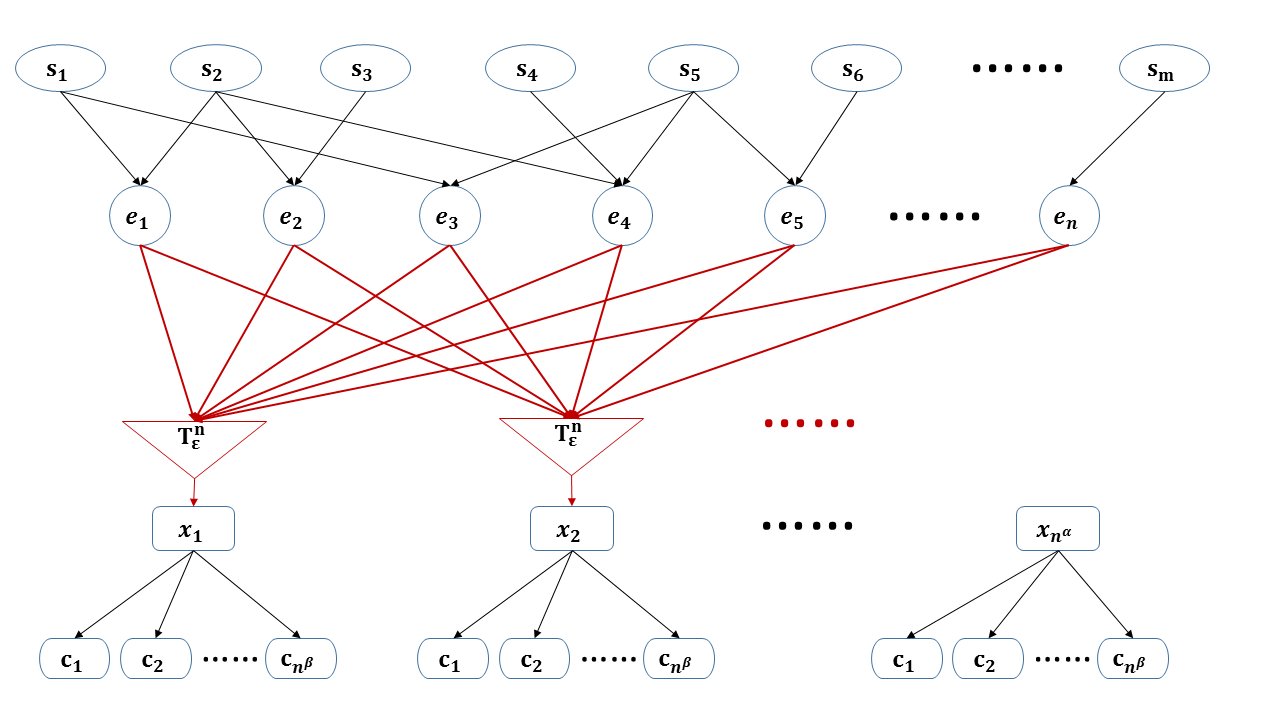
\includegraphics[width=\textwidth]{inapp_structure.png}
	\caption{集合覆盖构造$\varepsilon$-次模近似图}\label{fig:inapp_structure}
\end{figure}
然后对于参数$\alpha$,我们对每一个与门节点$x_k$添加$n^\alpha$个冗余节点$c_1, c_2, \dots, c_{n^\beta}$。
对每个冗余节点$c_l$,阈值函数同样是$f_{c_l}(1)=1$。
构建好的图中有集合节点$s_i$,元素节点$e_j$,与门节点$x_k$,冗余节点$c_l$以及构成概率与门的节点。
除了构成概率与门的节点阈值函数是等式\ref{eq:func_g}定义的$\varepsilon$-次模逼近函数,其余节点的阈值函数都是次模函数。
图\ref{fig:inapp_structure}中红色的边代表着概率与门中节点的阈值函数是$\varepsilon$-次模逼近函数。

接下来我们计算$T_\varepsilon^n$的深度,需要$T_\varepsilon^n$足够深才能以高概率保证$n^\alpha$个$T_\varepsilon^n$全部成功运作。
运行Union Bound,$n^\alpha$个$T_\varepsilon^n$至少有一个运作失败的概率至多是$n^{1+\alpha}(\frac{2-\varepsilon}{2})^{d}$。
令$d = (1+\alpha+\lambda)\log n / \log{\frac{2}{2-\varepsilon}}$,
在这个情况下所有概率与门$T_\varepsilon^n$均成功运作的概率至少是$1-n^{-\lambda}$。

如果我们能找到$k$个集合覆盖住所有$n$个元素,那么在这个构造的图中我们把对应那$k$个集合的节点选作种子节点。
接下来种子节点会激活所有的元素节点$e_1, e_2, \dots, e_n$,然后$T_\varepsilon^n$中的所有节点都会被激活。
最终,所有的与门节点$x_1, x_2, \dots, x_{n^\alpha}$以及他们指向的冗余节点都会被激活,一共被激活的节点个数是
$$k+n+n^{\alpha+1}(2^d-1)+n^{\alpha\beta} \geq n^{\alpha\beta}.$$
整个图中一共有
$$k+n+n^{\alpha+1}(2^d-1)+n^{\alpha\beta} \geq n^{\alpha\beta}$$
个节点,几乎图中所有的节点都会被激活。
另一方面,如果集合覆盖实例没有大小为$k$的解,就不能激活所有的元素节点$e_j$。
影响力传播过程中与门节点$x_1, x_2, \dots, x_{n^\alpha}$以高概率概率$1-n^{-\lambda}$都不会被激活。
此时,为了提升影响力,可以选择把与门节点$x_j$作为种子节点或者尽可能多的去激活元素节点$e_j$。
如果选择与门节点作为种子则最终激活至多$k+n+kn^{\beta}$个节点。
或者最多激活$n-1$个元素节点并激活几乎所有在概率与门机关中的$\varepsilon$-次模逼近节点,
这种情况下以高概率所有与门机关成功运作,最多$k+n-1+n^{\alpha+1}(2^d-1)$个节点会被激活。
如果概率与门运作失败,就假设此时所有节点最终都被激活。

现在我们设置参数$\alpha$和$\beta$,可以$\delta>0$取令$n^{\beta} = n^{\alpha-1} \cdot 2^d \cdot n^{\delta}$。
此时与门机关中节点的个数和冗余节点个数的比值为$n^{\alpha+1}(2^d-1) / n^{\alpha\beta} < n^{\frac{1}{\alpha-1}}$。
当$n$区域无穷时,如果集合覆盖问题无解,影响力范围以高概率$1-n^{-\lambda}$不会超过$kn^{\beta} \leq n^{\beta+1}$和$n^{\alpha+1}2^d$。
也就是说对于任意的影响力最大化算法,存在一个$N$个节点的图,其中至多有$n^{\alpha+1}(2^d-1)$个$\varepsilon$-次模逼近节点,
而对于算法输出的种子集合,以$1-n^{-\lambda}$的概率影响力不会超过$kn^{\beta} \leq n^{\beta+1}$和$n^{\alpha+1}2^d$,
除非集合覆盖问题有多项式时间的算法(NP=P)。
在这个图中,最优的种子集合$S^*$的影响力几乎是$N$,可以得到近似比不会超过
\begin{equation}
\label{eq:inapp_ratio}
\begin{array}{ll}
& \frac{\max\{kn^{\beta}, n^{\alpha+1}2^d\} * (1-n^{-\lambda}) + n^{-\lambda} * \sigma(S^*)}{\sigma(S^*)} \\
\leq & n^{-\lambda} + 
\frac{\max\{n^{\beta+1}, n^{\alpha+1}2^d\} * (1-n^{-\lambda})}
{k+n+n^{\alpha+1}(2^d-1)+n^{\alpha\beta} \geq n^{\alpha\beta}} \\
\leq & n^{-\lambda} + n^{-(\alpha-1)}
\end{array}
\end{equation}
这里$N \geq n^{\alpha+\beta}$,与门机关的深度为$d = (1+\alpha+\lambda)\log n / \log{\frac{2}{2-\varepsilon}}$,
参数$\beta = (\alpha+1) + (1+\alpha+\lambda) / \log{\frac{2}{2-\varepsilon}} + \delta$。
我们把参数带入不等式\ref{eq:inapp_ratio}和上述描述,得到
对于任意的$\alpha>1, \lambda>0, \delta>0$,存在$b = 1/\log{\frac{2}{2-\varepsilon}}$
$\varphi= \frac{ \min\{\alpha-1, \lambda\}}{2\alpha+\delta-1+b(1+\alpha+\lambda)}$和
$\gamma =\frac{\alpha+1+b(1+\alpha+\lambda)}{2\alpha+\delta-1+b(1+\alpha+\lambda)}$,
任意的基于$(\gamma,\varepsilon)$-次模逼近图的影响力最大化算法,
都可以构造出一个$\varepsilon$-次模逼近图实例,在这个图上算法的近似比不会超过$n^{-\gamma}$。
注意到这里$\varphi \geq \frac{\gamma}{3+3b}$在我们设定 $\alpha=\lambda+1$且$\lambda \geq 1$时。
$\gamma$的取值范围是$(0,1)$,也就是对于任意比例的$\varepsilon$-次模逼近节点结论都成立。
至此,我们证明了定理\ref{the:inapp}。
\end{proof}

\section{基于上下届的近似算法}
在前一小节,我们证明了$\varepsilon$-次模逼近节点较多时影响力最大化算法很难近似。
在本小姐,我们讨论图中只有比较少的$\varepsilon$-次模逼近节点的情况,通常是常数个或者$\log n$个。
首先我们提供了基于图中有较少非次模节点的朴素的贪心算法,
然后把非次模节点的阈值函数限定为$\varepsilon$-次模逼近并进一步提升了算法效果。


\subsection{非次模节点较少图的近似算法}
对于有$\ell (\ell<k)$个非次模节点的图,我们提供如下的近似算法。
\begin{algorithm}[h]
	\caption{\textbf{Naive-Greedy(G,k)}: Greedy for graph with $\ell$ non-submodular nodes.}
	\label{alg:naive_greed} 
	\begin{algorithmic}[1]
		\Require $G$: social graph of general threshold model, $k$: budget of seeds.
		\Ensure selected seed set $S$.
		\State Initialize $S = \emptyset$
		\ForAll { non-submodular node $v$}
			\State $S = S \cup \{v\}$
		\EndFor
		\For {$i=1$ to $k - \ell$}
			\State $v = \mathrm{argmax}_{u \in V \setminus S}$ \Call{MC-Spread}{$S \cup \{u\}, G$}
			\State $S = S \cup \{u\}$
		\EndFor
		\State \Return $S$
	\end{algorithmic} 
\end{algorithm}
在Algorithm\ref{alg:naive_greed}中,首先把所有的非次模节点加入种子集合,然后再依据贪心策略添加余下的$k - \ell$节点。
接下来分析算法的性能:


\begin{theorem}\label{the:naive_greedy}
给定一个$n$个节点的图$G$,其中除了$\ell < k$个节点的阈值函数是非次模函数,其余节点的阈值函数均是次模。
在图$G$上的影响力最大化算法Algorithm\ref{alg:naive_greed}可以取得$(1-e^{-\frac{k-\ell}{k}})(1-\frac{1}{e})$的近似比。
\end{theorem}
\begin{proof}
假设$S^*$是图$G$影响力最大化的最优种子集合,$V_e$是$\ell$个阈值函数非次模的节点集合,
令$S^*_{V_e} = S^* \cup V_e$。
很显然,由于影响力函数$\sigma(\cdot)$是单调非减的$\sigma(S^*_{V_e}) \geq \sigma(S^*)$。
由于$V_e$中的节点阈值函数是非次模的,所以我们不能直接应用贪心策略去做。
但是把$V_e$加入到种子节点后,函数$\sigma(S\cup V_e)$对于输入$S \subseteq V-V_e$来说是满足次模性质的。

通过预先把$V_e$中的节点加入种子集合,然后再通过贪心策略添加$k$个种子得到一个大小为$k+\ell$的种子集合$S^g_{V_e,k}$。
贪心策略有$1-\frac{1}{e}$的近似比,所以$\sigma(S^g_{V_e,k}) \geq (1-\frac{1}{e})\sigma(S^*_{V_e})$。
我们假设$S^*_{V_e}=V_e \cup \{s_1,s_2,\dots,s_{k'}\}, k'\leq k$, 其中$s_i \not\in V_e$是不属于$V_e$的节点。
令$S_i = \{s_1,s_2,\dots,s_i\}$。
实际上,根据$1-1/e$近似比的证明过程,对于$i\leq k$我们有:
\begin{equation}
\label{eq:1e_proof}
\begin{array}{ll}
&\sigma(S^*_{V_e})\\
\leq & \sigma(S^*_{V_e} \cup S^g_{V_e,i})\\
= & \sigma(S^g_{V_e,i}) +
	\sum_{j=1}^{k'} \big( \sigma(S^g_{V_e,i} \cup S_j) - 	
	\sigma(S^g_{V_e,i} \cup S_{j-1})\big)\\
\leq & \sigma(S^g_{V_e,i}) +
	\sum_{j=1}^{k'} \big( \sigma(S^g_{V_e,i} \cup \{s_j\}) - 	
	\sigma(S^g_{V_e,i})\big)\\
\leq & \sigma(S^g_{V_e,i}) +
	k\cdot \big( \sigma(S^g_{V_e,i+1})-\sigma(S^g_{V_e,i})\big)\\
\end{array}
\end{equation}
不等式\ref{eq:1e_proof}的第一行是因为影响力函数$\sigma$是单调非减的,
第三行是因为$\sigma$是次模函数。
不等式\ref{eq:1e_proof}第四行成立的原因是$S^g_{V_e,i+1}$是基于贪心算法
在$S^g_{V_e,i}$的基础上选出的边际影响力最大的节点,边际影响力要大于节点$s_{i+1}$。
然后我们可以得到:
\begin{equation*}
\label{eq:sub_greedy_re}
\begin{array}{ll}
\sigma(S^*_{V_e}) - \sigma(S^g_{V_e,i}) \leq
k\cdot \big( \sigma(S^g_{V_e,i+1})-\sigma(S^g_{V_e,i})\big) \\
\sigma(S^*_{V_e}) - \sigma(S^g_{V_e,i+1}) \leq
(1-\frac{1}{k}) \big( \sigma(S^*_{V_e}) - \sigma(S^g_{V_e,i}) \big)
\end{array}
\end{equation*}
如果只使用贪心策略选择$k-\ell$个节点的话,
\begin{equation*}
\begin{array}{ll}
& \sigma(S^*_{V_e}) - \sigma(S^g_{V_e,k-\ell}) \\
\leq & (1-\frac{1}{k})^{k-\ell} (\sigma(S^*_{V_e}) - \sigma(V_e))\\
\leq & (1-\frac{1}{k})^{k-\ell} \sigma(S^*_{V_e})
\end{array}
\end{equation*}
公司的第二行是重复使用不等式\ref{eq:sub_greedy_re}。
所以在种子集合加入$V_e$后再选择$k-\ell$个种子的情况下,
$$\sigma(S^g_{V_e,k-\ell})
\geq (1-(1-\frac{1}{k})^{k-\ell}) \sigma(S^*_{V_e})
\geq (1-e^{-\frac{k-\ell}{k}}) \sigma(S^*)$$

所以先把非次模节点加入种子集合,然后再贪心的选择$k-\ell$个种子节点,依然可以得到一个近似比$(1-e^{-\frac{k-\ell}{k}})$的解,定理证明完毕。
\end{proof}

Algorithm\ref{alg:naive_greed}有一定局限性,非次模节点个数不能太多,不能超过给定的$k$。
然后算法也只能粗暴的把非次模节点加入种子集合来保证次模性质,非次模节点个数较多时算法近似比很差。
同时算法对于非次模节点的阈值函数没有限制,在阈值函数是$\varepsilon$-次模时不能提升效果。

\subsection{基于次模上下界的近似算法}
在前一小节,本文提供了一个简单的针对图中有$\ell~(\ell<k)$个非次模节点的影响力最大化近似算法。
在本节,我们考虑非次模函数是$\varepsilon$-次模逼近函数的情况,提供了一个基于$\varepsilon$-次模逼近图的近似算法,并证明了算法的近似比。
整体思路是概率空间的映射。

在定义\ref{def:eas}中,我们定义了$\varepsilon$-次模逼近函数$f_v$的次模上界函数$\overline{f}_v$和次模下界函数$\underline{f}_v$。
注意到次模函数也是$\varepsilon$-次模逼近,对次模函数$f_v$来说,$\underline{f}_v = f = (1-\varepsilon)\overline{f}_v$。
根据定义,可以推出对于任意的输入$\underline{f}_v \geq (1-\varepsilon)\overline{f}_v$。
给定一个包含$\varepsilon$-次模逼近节点的图,我们可以把每个节点的阈值函数替换成次模下界函数,
然后在新构建的图上运行经典的基于次模的影响力最大化算法(Algorithm~\ref{alg:Galg_L})。
下面的定理证明了这种贪心算法的近似比。

\begin{algorithm}[h]
	\caption{\textbf{Galg-L($G,k,\mathcal{A},\{\overline{f}_v\},\{\underline{f}_v\}$)}: algorithm for zoomed threshold model.}
	\label{alg:Galg_L} 
	\begin{algorithmic}[1]
		\Require $G$: social graph, $k$: budget of seeds, $\mathcal{A}$: greedy IM algorithm, 
			$\{\overline{f}_v\},\{\underline{f}_v\}$: submodular upper and lower function.
		\Ensure selected seed set $S$.
		\State Initialize $S = \emptyset$
		\State replace each nodes $v$'s threshold function $f_v$ with $\underline{f}_v$
		\State run greedy algorithm $\mathcal{A}$ on $G$ with $\{\underline{f}_v\}$ and obtain $S$
		\State \Return $S$
	\end{algorithmic} 
\end{algorithm}


\begin{theorem}
\label{thm:app_alg}
给定通用阈值模型的一个图$G$,
如果图中只有$c$个节点的阈值函数是$\varepsilon$-次模逼近而其余节点的阈值函数均是次模,
那么算法{\bf Galg-L}可以输出近似比为$(1-\frac{1}{e})(1-\varepsilon)^c$的种子集合。
\end{theorem}
\begin{proof}
令$V_e$为$\varepsilon$-次模逼近节点的集合。
不失一般性,我们可以假设$V_e = \{v_1,v_2,\dots,v_c\}$。
现在考虑这两个阈值函数均为次模函数的图$\overline{G}, \underline{G}$,它们的节点和图$G$一致.
这两个图中每个节点$v$的阈值函数分别是$\overline{f}_v$和$\underline{f}_v$。
图$G$、$\overline{G}$和$\underline{G}$中,$V-V_e$内的节点阈值函数相同,
$V_e$内节点的阈值函数分别为$\varepsilon$-次模逼近、次模上界和次模下界函数。

对于通用阈值模型来说,如果每个节点$v$的阈值$\theta_v$都被确定了,传播过程就变成了确定性的。
一个阈值函数为$\{f_v\}$的图$G$和给定的节点阈值$\{\theta_v\}$被称为{\it 可能世界图}(possible world),
这和独立级联模型的活边子图(live-edge graph)很类似。
一个可能世界图可以被表示为
$$\{\theta_{v_1},\theta_{v_2},\dots,\theta_{v_n};f_{v_1},f_{v_2},\dots,f_{v_n}\}$$
分别是每个节点的阈值和阈值函数。
这里我们通过$\theta_{v}\leq 1-\varepsilon (v\in V_e)$构建$\underline{G}$和$\overline{G}$之间可能世界图的一一映射。

\begin{equation}
\label{eq:possible_world}
\begin{array}{ll}
\{\theta_{v_1},\dots,\theta_{v_c},\theta_{v_{c+1}}\dots,\theta_{v_n};
f_{v_1}, \dots,f_{v_n}\} \leftrightarrow \\
\{\frac{\theta_{v_1}}{1-\varepsilon},\dots,\frac{\theta_{v_1}}{1-\varepsilon},\theta_{v_{c+1}}\dots,\theta_{v_n};
\frac{f_{v_1}}{1-\varepsilon},\dots,\frac{f_{v_c}}{1-\varepsilon},f_{v_{c+1}},\dots,f_{v_n}\} \\
\end{array}
\end{equation}

等式\ref{eq:possible_world}描述了$\underline{G}$和$\overline{G}$的一一映射。
给定$\underline{G}$的任意可能世界图,
对于任意在$V_e$中的节点$v\in V_e$且阈值$\theta_{v}\leq 1-\varepsilon$,
把阈值$\theta_{v}$放大至$\frac{\theta_{v}}{1-\varepsilon}$。
与此同时,也把这些节点的阈值函数也放大$\frac{1}{1-\varepsilon}$倍到$\frac{f_{v}}{1-\varepsilon}$。
显然,这个放大过程不会影响在可能世界图中的传播过程,
但是放大之后$\underline{G}$的可能世界图变成了$\overline{G}$中的一个可能世界。

期望的影响力$\sigma$可以通过对阈值积分计算:
$$\sigma(S)=\int_{\mathbb{\theta}\in[0,1]^n} \mathcal{D}(\mathbb{\theta};f,S) \mbox{d}_{\mathbb{\theta}}$$
$\mathcal{D}(\mathbb{\theta};f,S)$代表的是在可能世界图$(\mathbb{\theta};f)$中种子集合$S$确定的的影响力大小。
称图$\overline{G},\underline{G}$的影响力函数分别为$\overline{\sigma},\underline{\sigma}$。
定义$\vec{\theta}\in[0,1]^n$为$n$个节点阈值组成的$n$维向量,
$\vec{\theta}_e \in[0,1]^{c}$和$\vec{\theta}'\in[0,1]^{n-c}$分别是集合$V_e$和$V-V_e$的阈值向量。
类似的可以定义阈值函数向量,定义$V_e$和$V-V_e$的阈值函数向量分别为$\vec{f}_e,\vec{f}'$。
一个可能世界图被简写为:
$$\{\vec{\theta}_e,\vec{\theta}';\vec{f}_e,\vec{f}'\}$$
对于任意的种子集合,可以得到:
\begin{equation}
\label{eq:sigma_geq}
\begin{array}{ll}
&\underline{\sigma}(S)\\
=&\int_{\vec{\theta}\in[0,1]^n} \mathcal{D}(\vec{\theta};\vec{f},S) \mbox{d}_{\vec{\theta}} \\
\geq&\int_{\vec{\theta}_e\in[0,1-\varepsilon]^c}\int_{\vec{\theta}'\in[0,1]^{n-c}} \mathcal{D}(\vec{\theta}_e,\vec{\theta}';\vec{f},S) \mbox{d}_{\vec{\theta}_e}\mbox{d}_{\vec{\theta}'} \\
=&(1-\varepsilon)^c \int_{\frac{\vec{\theta}_e}{1-\varepsilon}\in[0,1]^c}\int_{\vec{\theta}'\in[0,1]^{n-c}} \mathcal{D}(\vec{\theta}_e,\vec{\theta}';\vec{f},S) \mbox{d}_{\frac{\vec{\theta}_e}{1-\varepsilon}}\mbox{d}_{\vec{\theta}'} \\
=&(1-\varepsilon)^c \int_{\frac{\vec{\theta}_e}{1-\varepsilon}\in[0,1]^c}\int_{\vec{\theta}'\in[0,1]^{n-c}} \mathcal{D}(\frac{\vec{\theta}_e}{1-\varepsilon},\vec{\theta}';\frac{\vec{f}_e}{1-\varepsilon},\vec{f}',S) \mbox{d}_{\frac{\vec{\theta}_e}{1-\varepsilon}}\mbox{d}_{\vec{\theta}'} \\
=&(1-\varepsilon)^c \int_{\vec{\theta}\in[0,1]^n} \mathcal{D}(\vec{\theta};\frac{\vec{f}_e}{1-\varepsilon},\vec{f}',S) \mbox{d}_{\vec{\theta}} \\
=&(1-\varepsilon)^c \overline{\sigma}(S).\\
\end{array}
\end{equation}
不等式\ref{eq:sigma_geq}的第三个等号利用了$\underline{G}$和$\overline{G}$可能世界图的一一映射。
因此,给定一个种子集合$S$,在图$\overline{G}$和图$\underline{G}$中对应的影响力函数满足关系:
$$\underline{\sigma}(S) \geq (1-\varepsilon)^c \overline{\sigma}$$



称$\sigma$为原图$G$的影响力函数,令$\overline{S}^*,S^*,\underline{S}^*$分别代表
$\overline{\sigma}, \sigma, \underline{\sigma}$的影响力最大化问题最优解。
显然$\overline{\sigma}(\overline{S}^*) \geq \sigma(S^*)$,因为对任意节点$v$都有$\overline{f}_v \geq f_v$。
根据前文的不等式\ref{eq:sigma_geq},推出
$$\underline{\sigma}(\underline{S}^*)
\geq \underline{\sigma}(\overline{S}^*)
\geq (1-\varepsilon)^c \overline{\sigma}(\overline{S}^*)$$
因此对于基于$\overline{\sigma}$的贪心算法$\mathcal{A}$的输出种子集合$S^{\mathcal{A}}$,有近似比如下:
\begin{equation*}
\begin{array}{ll}
& \sigma(S^{\mathcal{A}}) \\
\geq & \underline{\sigma}(S^{\mathcal{A}}) \\
\geq & (1-\frac{1}{e})\underline{\sigma}(\underline{S}^*)\\
\geq & (1-\frac{1}{e})(1-\varepsilon)^c \overline{\sigma}(\overline{S}^*) \\
\geq &(1-\frac{1}{e})(1-\varepsilon)^c \sigma(S^*) \\
\end{array}
\end{equation*}
至此定理证明完毕。
\end{proof}

如果Algorithm~\ref{alg:Galg_L}$\varepsilon$-次模逼近函数替换成对应的上界然后运行贪心算法,
可以得到类似的结果,近似比也是$(1-\frac{1}{e})(1-\varepsilon)^c$,我们称这种算法为\textbf{Galg-L}。
证明过程中用到的技巧和Lu等人\cite{lu2015competition}的{\em sandwich approximation}有些相似。
但是他们的近似比依赖于尚未确定的影响力大小,而我们的工作利用概率空间映射直接求出了近似比的数值。


\section{本章小结}
本章主要讨论了$\varepsilon$-次模逼近网络中影响力最大化问题,
给出了图中有$n$的多项式个$\varepsilon$-次模逼近节点时的不可近似性,
最后分别基于贪心策略和概率空间映射策略设计了两个近似算法,各自分析了近似比。
4.1节分析讨论了$n$个节点的图中有$n^{\gamma}$个$\varepsilon$-次模逼近节点的情况,基于机关构造从NP完全问题集合覆盖给出了不可近似性证明的规约。
4.2节首先给出针对图中有常数个非次模节点的近似算法,然后基于$\varepsilon$-次模逼近函数的次模上下界设计了近似算法,通过概率空间映射给出近似比证明。







